% A LaTeX (non-official) template for ISAE projects reports
% Copyright (C) 2014 Damien Roque
% Version: 0.2
% Author: Damien Roque <damien.roque_AT_isae.fr>

\documentclass{beamer}
\usepackage[utf8]{inputenc}
\usepackage[frenchb]{babel}
\usepackage{palatino}
\usepackage{graphicx}
\graphicspath{{./images/}}
\usepackage{colortbl}
\usepackage{xcolor}
\usepackage{tikz}
\usetikzlibrary{shapes,arrows}
\usetikzlibrary{mindmap,trees}
\usetikzlibrary{calc}
\usepackage{pgfplots}
\pgfplotsset{compat=newest}
\pgfplotsset{plot coordinates/math parser=false}
\newlength\figureheight
\newlength\figurewidth
\usepackage{ifthen}
\usepackage{subfigure}
\usepackage{amsthm}
\usepackage{amsfonts}
\usepackage{amssymb}
\usepackage{amsmath}
\usepackage{eurosym}
\usepackage{wasysym}
\usepackage{wrapfig}
\usepackage{dsfont}
% Printing on 2 slides per page
%\pgfpagesuselayout{2 on 1}[a4paper,border shrink=5mm]

% My macros...
\newcommand*{\SET}[1]  {\ensuremath{\boldsymbol{#1}}}
\newcommand*{\VEC}[1]  {\ensuremath{\boldsymbol{#1}}}
\newcommand*{\MAT}[1]  {\ensuremath{\boldsymbol{#1}}}
\newcommand*{\OP}[1]  {\ensuremath{\text{#1}}}
\newcommand*{\NORM}[1]  {\ensuremath{\left\|#1\right\|}}
\newcommand*{\DPR}[2]  {\ensuremath{\left \langle #1,#2 \right \rangle}}
\newcommand*{\calbf}[1]  {\ensuremath{\boldsymbol{\mathcal{#1}}}}
\newcommand*{\shift}[1]  {\ensuremath{\boldsymbol{#1}}}
\newcommand{\eqdef}{\stackrel{\mathrm{def}}{=}}
\newcommand{\argmax}{\operatornamewithlimits{argmax}}
\newcommand{\argmin}{\operatornamewithlimits{argmin}}
\newcommand{\ud}{\, \text{d}}
\newcommand{\vect}{\text{Vect}}
\newcommand{\sinc}{\text{sinc}}
\newcommand{\esp}{\ensuremath{\mathbb{E}}}
\newcommand{\hilbert}{\ensuremath{\mathcal{H}}}
\newcommand{\fourier}{\ensuremath{\mathcal{F}}}
\newcommand{\sgn}{\text{sgn}}
\newcommand{\intTT}{\int_{-T}^{T}}
\newcommand{\intT}{\int_{-\frac{T}{2}}^{\frac{T}{2}}}
\newcommand{\intinf}{\int_{-\infty}^{+\infty}}
\newcommand{\Sh}{\ensuremath{\boldsymbol{S}}}
\newcommand{\Cpx}{\ensuremath{\mathbb{C}}}
\newcommand{\R}{\ensuremath{\mathbb{R}}}
\newcommand{\Z}{\ensuremath{\mathbb{Z}}}
\newcommand{\N}{\ensuremath{\mathbb{N}}}
\newcommand{\K}{\ensuremath{\mathbb{K}}}
\newcommand{\reel}{\mathcal{R}}
\newcommand{\imag}{\mathcal{I}}
\newcommand{\cmnr}{c_{m,n}^\reel}
\newcommand{\cmni}{c_{m,n}^\imag}
\newcommand{\cnr}{c_{n}^\reel}
\newcommand{\cni}{c_{n}^\imag}
\newcommand{\LR}{\mathcal{L}_2(\R)}
\newcommand{\tproto}{g}
\newcommand{\rproto}{\check{g}}
\newcommand{\Tproto}{G}
\newcommand{\Rproto}{\check{G}}


\setbeamertemplate{itemize item}[ball]


%\theoremstyle{definition}
%\newtheorem{definition}{Définition}[subsection]

\theoremstyle{remark}
\newtheorem{remarque}{Remarque}[subsection]

\theoremstyle{plain}
\newtheorem{propriete}{Propriété}[subsection]
\newtheorem{exemple}{Exemple}[subsection]

% Choosing a main theme and a color theme
\mode<presentation> {
    \setbeamertemplate{background canvas}[vertical shading][bottom=white!10,top=blue!10]
  %\usetheme{Warsaw}
  \usetheme{Madrid}
  %\usetheme{Frankfurt}
  %\usecolortheme{seahorse}
}


\addtobeamertemplate{frametitle}{}{%
\vskip-1em
\begin{tikzpicture}[remember picture,overlay]
\node[anchor=north east,yshift=4pt] at (current page.north east) {
\includegraphics[height=0.85cm]{images/telecomnancy.png}};
\end{tikzpicture}}

\title[Stage 2A]{Analyse exploratoire des données spatialisées en utilisant des processus ponctuels}

\author[C. Dugué]{\small Clément Dugué}%\inst{1} }

%\date{23 janvier 2014}

\institute[TELECOM NANCY]
{
\vspace{0.25cm}


\includegraphics[height=1.5cm]{images/universitelorraine.jpg}
\hspace{0.5cm}

\includegraphics[height=1.5cm]{images/telecomnancy.png}
\hspace{0.5cm}

\includegraphics[height=1.5cm]{images/iecl.png}\\

 \begin{center}
    \vspace{1em}
    Stage de 2ème anné encadré par Radu Stoica\\
 \end{center}
 
}
% Clear the navigation bar
\setbeamertemplate{navigation symbols}{}
 
\subject{Sujet de la présentation}

\begin{document}

\begin{frame}
\titlepage
\end{frame}

\begin{frame}
  \frametitle{Plan}
  \small
  \tableofcontents
  \normalsize
\end{frame}

% Recall the outline at each section
%\AtBeginSection[]
%{
%\begin{frame}
%  \frametitle{Plan}
%  \small
%  %\tableofcontents[hideothersubsections]
%  \tableofcontents[currentsubsection,hideothersubsections]
%  %\tableofcontents[currentsubsection]
%  \normalsize
%\end{frame}
%}

%%%%%%%%%%%%%%%%%%%%%%%%%%%%%%%%%%%%%

\section{Introduction}
\label{sec:partie1}

\subsection{Présentation de l'entreprise}
\begin{frame}
  \frametitle{Présentation de l’entreprise}
  \vspace{-1cm}
  \begin{center}
  
\includegraphics[height=1.5cm]{images/universitelorraine.jpg}
  \hspace{0.5cm}
  
\includegraphics[height=1.5cm]{images/iecl.png}
  \hspace{0.5cm}
  
\includegraphics[height=1.5cm]{images/cnrs.jpeg}
  \vspace{1cm}
  \hspace{2cm}
  \begin{itemize}
        \item{Recherche en Lorraine} 
        \vspace{0.5cm}
        \item{Institut Elie Cartan} 
        \vspace{0.5cm}
        \item{Equipe Probabilités et Statistiques}
  \end{itemize}
  \end{center}
\end{frame}

\subsection{Contexte du stage}
\begin{frame}
  \frametitle{Contexte du stage}
   \hspace{0.2cm}
  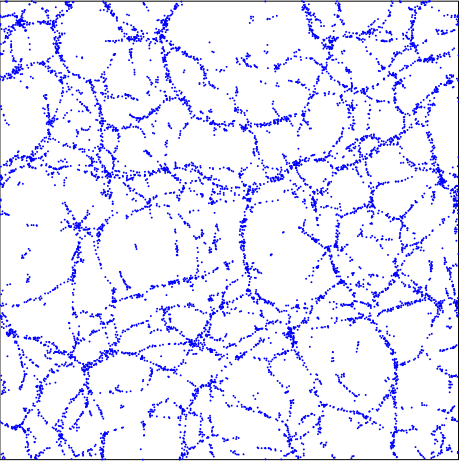
\includegraphics[height=5cm]{images/exempleConfiguration.png}
  %\vspace{0.5cm}
  \hspace{0.5cm}
  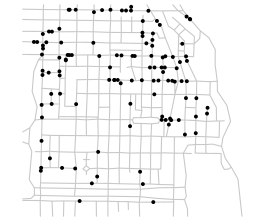
\includegraphics[height=5cm]{images/crimesChicago.png}\\
  
  \begin{columns}
    \begin{column}{0.45\linewidth}
      \begin{center}
        %\\
        Exemple de configuration de point - Jeu de données fourni par M. Stoica
      \end{center}
    \end{column}
    \begin{column}{0.45\linewidth}
      \begin{center}
        Crimes sur 2 semaines dans les environs de l'Université de Chicago \cite{BaddEtal16}
      \end{center}
    \end{column}
  \end{columns}
  
  
\end{frame}

%%%%%%%%%%%%%%%%%%%%%%%%%%%%%%%%%%%%%

\section{Cahier des charges du projet}
\label{sec:partie2}

\subsection{Fonctions à réaliser}
\begin{frame}
    \frametitle{Fonctions à réaliser}
    \begin{itemize}
    \item{K : moyenne normalisée du nombre de voisin \\
        \hspace{4cm}
        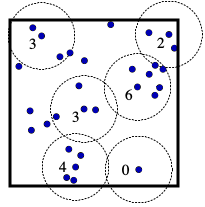
\includegraphics[height=2.5cm]{images/nombreVoisins2.png}
    } 
    \item{F : fonction d'espace vide 
      \begin{equation}
        F(r) = \mathbb{P}\{ d(u,\textbf{x}) \leq r \} 
      \end{equation}
    }
    \item{G : fonction du plus proche voisin 
    \begin{equation}
        G(r) = \mathbb{P}\{ d(u,\textbf{x}\backslash u) \leq r | \text{ u est un point de \textbf{x}} \} 
      \end{equation}
    }
    \item{J :
      \begin{equation}
        J(r) = \frac{1-G(r)}{1-F(r)}
      \end{equation}
    }
  \end{itemize}
\end{frame}

\subsection{Insertion dans un code existant}
\begin{frame}
    \frametitle{Insertion dans un code existant}
    \vspace{-0.5cm}
    \begin{columns}
    \begin{column}{0.3\linewidth}
        \begin{itemize}
            \item{Test d'enveloppe} 
             \vspace{0.5cm}
            \item{"Strauss"} 
             \vspace{0.5cm}
            \item{"Area Interaction"}
        \end{itemize}
    \end{column}
    \begin{column}{0.45\linewidth}
      \begin{center}
        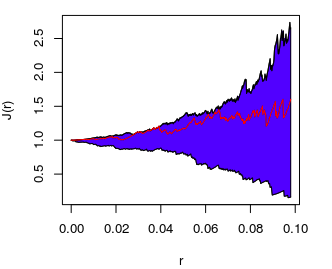
\includegraphics[width=6cm]{images/enveloppeJ.png}\\
        Exemple d'enveloppe pour la fonction J avec la méthode "Strauss"
      \end{center}
    \end{column}
  \end{columns}
\end{frame}

\subsection{Travail supplémentaire: l'intensité}
\begin{frame}
    \frametitle{Travail supplémentaire: l'intensité}
      \begin{center}
        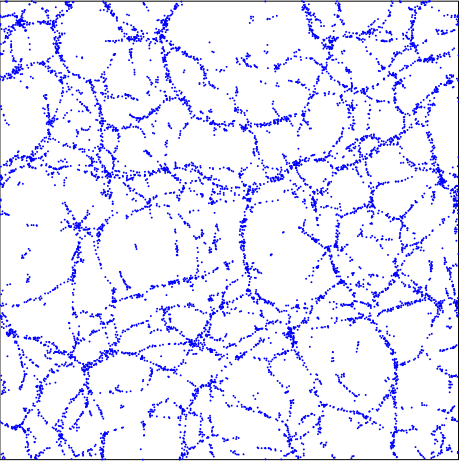
\includegraphics[width=4.4cm]{images/exempleConfiguration.png}
        \hspace{0.5cm}
        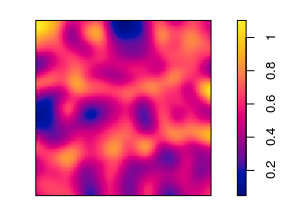
\includegraphics[width=5.7cm]{images/intensiteSpatstat.png}\\
        Exemple d'intensité calculée à partir de la configuration de point à gauche - Créée avec la librairie R-Spatstat%~\cite{FAQspatstat}
      \end{center}
    
\end{frame}

%%%%%%%%%%%%%%%%%%%%%%%%%%%%%%%%%%%%%

\section{Méthode de travail}
\label{sec:partie3}

\subsection{Outils utilisés}
\begin{frame}
    \frametitle{Outils utilisés}
    
\includegraphics[height=1.5cm]{images/cpp_logo.png}
    \begin{itemize}%[label=triangle]
        \item{langage utilisé par mon tuteur}
        \item{langage orienté objet}
    \end{itemize}
    \vspace{0.5cm}
    
\includegraphics[height=1.5cm]{images/Rlogo.png}
    \begin{itemize}%[label=triangle]
        \item{adapté aux tests statistiques}
        \item{affichage des courbes}
    \end{itemize}
\end{frame}

\subsection{Manière de procéder}
\begin{frame}
  \frametitle{Manière de procéder}
  \begin{enumerate}
    \item{Assimilation de la théorie}
    \begin{itemize}%[label=triangle]
        \setbeamertemplate{itemize subitem}[triangle]
        \item{Lecture de la documentation}
        \item{Explications de M. Stoica}
    \end{itemize}
    \vspace{0.5cm}
    \item{Discutions avec le tuteur}
    \begin{itemize}%[label=triangle]
        \setbeamertemplate{itemize subitem}[triangle]
        \item{sur les structures de code à adopter}
        \item{sur les méthodes à utiliser}
    \end{itemize}
    \vspace{0.5cm}
    \item{Implémentation}
    \begin{itemize}%[label=triangle]
        \setbeamertemplate{itemize subitem}[triangle]
        \item{création des fonctions}
        \item{vérification des résultats (corrections si besoin)}
    \end{itemize}
  \end{enumerate}
\end{frame}

\subsection{Échanges avec le tuteur}
\begin{frame}
  \frametitle{Échanges avec le tuteur}
  \begin{itemize}
        \item{Un gros RDV par semaine}
        \begin{itemize}%[label=triangle]
            \setbeamertemplate{itemize subitem}[triangle]
            \item{Aide à la compréhension de la théorie}
            \item{Discutions sur les méthodes d'implémentaion}
            \item{Réponse aux questions}
            \item{Planification du travail}
        \end{itemize}
        \vspace{0.5cm}
        \item{Petites rencontres régulières}
        \begin{itemize}%[label=triangle]
            \setbeamertemplate{itemize subitem}[triangle]
            \item{Confirmations, validation du travail}
            \item{Petits changements / corrections}
            \item{Aide}
        \end{itemize}
  \end{itemize}
\end{frame}

%%%%%%%%%%%%%%%%%%%%%%%%%%%%%%%%%%%%%

\section{Solutions apportées et résultats}
\label{sec:partie4}

\subsection{Programmation des fonctions}
\begin{frame}
  \frametitle{Programmation des fonctions}
  % ou méthodes à choix 
  \begin{itemize}
        \item{fonction K:
        \begin{equation}
        K(r) = \frac{  \sum_{i=1}^n \mathds{1} \{b_i \geq r \} \sum_{\underset{j \neq i}{j=1}}^n \mathds{1} \{d_{ij} \leq r \}}{\lambda \sum_{i=1}^n \mathds{1} \{b_i \geq r \}}
        \end{equation}
        }
        
        \item{intensité:
        \begin{equation}
            \lambda(u) = \sum_{i=1}^n \frac{1}{ ( \int_W K(x_i-v) \, \mathrm dv )} k(u-x_i)
          \end{equation}
        }
        
        \item{adopter méthodes et stratégies pour implémentations optimales\\(tris, discrétisassion d'intégrales,...)}
  \end{itemize}
\end{frame}


\subsection{Automatisation}
\begin{frame}
  \frametitle{Automatisation}
    \begin{itemize}
        \item{Fichiers de sortie}\\
        \vspace{0.3cm}
        
\includegraphics[height=1.5cm]{images/fichierDeSortie.png}
        \vspace{0.5cm}
        \item{Scripts shell}\\
        \vspace{0.3cm}
        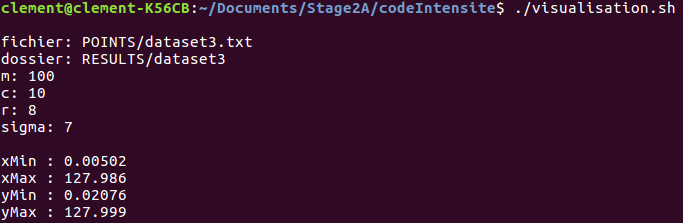
\includegraphics[height=3cm]{images/shell.png}
  \end{itemize}
\end{frame}

\subsection{Résultats}
\begin{frame}
  \frametitle{Résultats}
  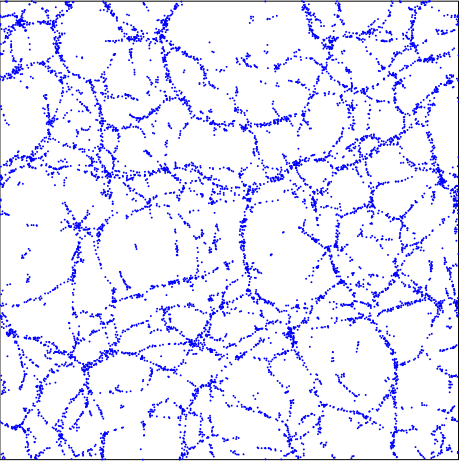
\includegraphics[height=5.5cm]{images/exempleConfiguration.png}
   \hspace{0.5cm}
  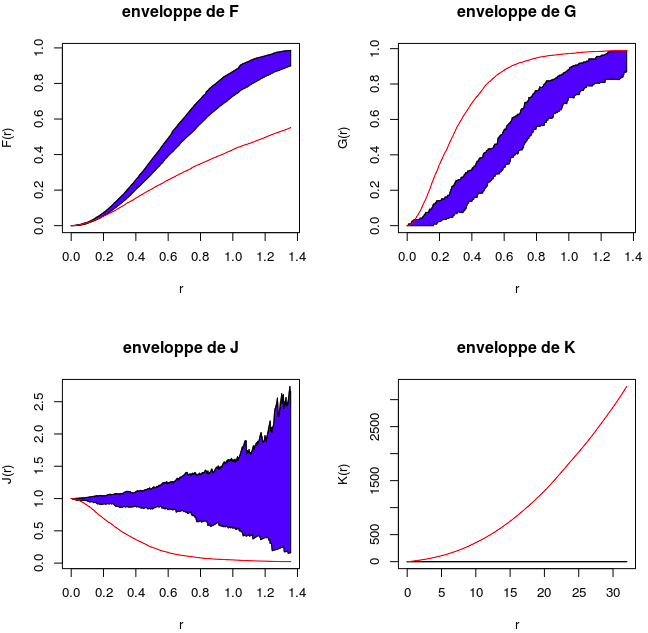
\includegraphics[height=5.5cm]{images/resultat.png}
\end{frame}

\begin{frame}
  \frametitle{Résultats}
  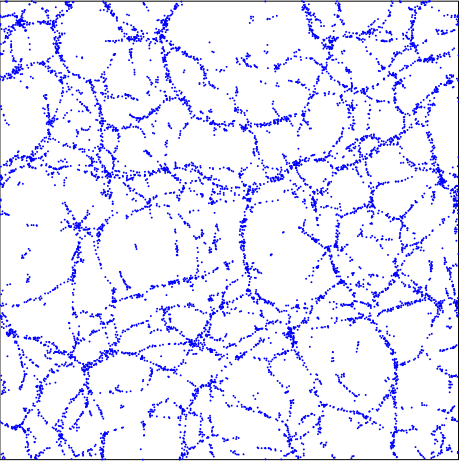
\includegraphics[height=5.5cm]{images/exempleConfiguration.png}
  \hspace{0.5cm}
  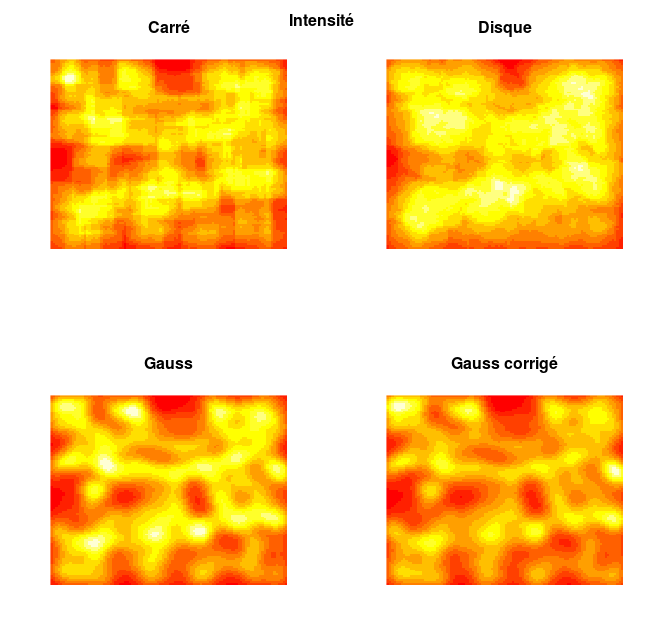
\includegraphics[height=5.5cm]{images/resultatIntensite.png}
\end{frame}
%%%%%%%%%%%%%%%%%%%%%%%%%%%%%%%%%%%%%

\section{Bilan du stage}
\label{sec:partie6}

\begin{frame}
  \frametitle{Bilan}
  
   \begin{itemize}
        \item{Projet impliquant un travail avec des personnes d'autres domaines scientifiques}
        \vspace{0.5cm}
        \item{Découverte ou approfondissement de domaines de connaissances}
        \begin{itemize}%[label=triangle]
            \setbeamertemplate{itemize subitem}[triangle]
            \item{en mathématique}
            \item{en informatique}
            \item{dans le domaine de la recherche}
        \end{itemize}
        \vspace{0.5cm}
        \item{Objectif atteint avec de nombreuses perspectives}%amélioration en code et décourverte d'un milieu
  \end{itemize}
  
  
   
\end{frame}


\begin{frame}
  \frametitle{Questions}
  \begin{center}
    Merci pour votre attention.

    Avez-vous des questions ?
  \end{center}
\end{frame}

\newcounter{lastframe}
\setcounter{lastframe}{\insertframenumber}

\begin{frame}[allowframebreaks]{References}
\bibliographystyle{authoryear-fr}
\bibliography{references}
\end{frame}

\setcounter{framenumber}{\thelastframe}

\end{document}
